63. $y=\cfrac{(x^2+2x-8)(x+2)}{|x+2|}=\begin{cases} x^2+2x-8,\ x>-2,\\ -x^2-2x+8,\ x<-2.\end{cases}$
$$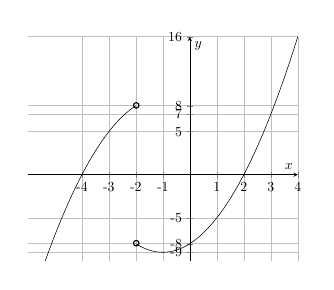
\begin{tikzpicture}[scale=0.5]
\begin{axis}[
    axis lines = middle,
    grid=major,
    legend pos={south west},
    xlabel = {$x$},
    %xlabel style={below right},
    ylabel = {$y$},
    ymin=-10,
    ymax=16,
    xmin=-6,
    xmax=4,
    xtick={-4,-2,-3,-1,1,2,3,4,6},
    xticklabels={-4,-2,-3,-1,1,2,3,4,6},
    ytick={-9,-8,-5,7,8,16,5},
    yticklabels={-9,-8,-5,7,8,16,5},
                  ]
	\addplot[domain=-6:-2, samples=100, color=black] {-(x*x+2*x-8)};
    \addplot[domain=-2:4, samples=100, color=black] {x*x+2*x-8};
    %\addplot[domain=2.01:6, samples=100, color=black] {2/(2-x)};
   % \addplot[domain=-3:3, samples=100, color=black] {-x};
     %\addlegendentry{$\text{Рис. 1}$};
\end{axis}
\draw (2.75,3.95) circle (2pt);
\draw (2.75,0.45) circle (2pt);
\end{tikzpicture}$$
По графику найдём $m\in(-9;-8).$\\
